%%%%%%%%%%%%%%%%%%%%%%%%%%%%%%%%%%%%%%%%%%%%%%%%%%%%%%%%%%%%%%%%%%%%%%%
%                                                                     %
%    MSc Project Proposal                                             %
%    Based on the UG/PG final report template by S.S. Oyelere         %
%    University of Exeter                                             %
%                                                                     %
%%%%%%%%%%%%%%%%%%%%%%%%%%%%%%%%%%%%%%%%%%%%%%%%%%%%%%%%%%%%%%%%%%%%%%%
\documentclass[11pt,a4paper]{article}

\usepackage{amsmath}
\usepackage{amsfonts}
\usepackage{geometry}
\usepackage{graphicx}
\usepackage{fancyhdr}
\usepackage{setspace}
\usepackage{amssymb}
\usepackage{booktabs}
\usepackage{enumitem}
\usepackage{multirow}
\usepackage{titlesec}
\usepackage{array}

% Figures live in the project's reports directory. Adjust if you move this file.
\graphicspath{{../../reports/phase9/}{./}}

% set table of content depth
\setcounter{tocdepth}{3}
\usepackage[titles]{tocloft}

% set spacing
\setlength{\cftbeforesecskip}{10pt}

% Page layout settings
\geometry{
    a4paper,
    left=20mm,
    right=20mm,
    top=25mm,
    bottom=25mm
}

%%%%%%%%%%%%%%%%%%%%%%%%%%%%%%%%%%%%%%%%%%%%%%%%%%%%%%%%%%%%%%%%%%%%%%
\begin{document}
\singlespacing
\thispagestyle{empty}

\begin{center}
{\bf \LARGE When Does a Machine-Learning Stage Earn Its Place?}\\[0.2cm]
{\bf \large A Rule-Grounded, Retrieval-Augmented System for Generating\\
Lifestyle Guidance from Blood-Test Reports}\\[0.6cm]
    \textbf{Bhavesh Bhargava} \\[0.2cm]
    \textbf{Student ID:} 1234567890 \\[0.2cm]
    \textbf{Programme:} MSc Advanced Data Science \\[1cm]
\end{center}

\section*{Abstract}

\noindent
Blood-test reports are returned to patients as tables of numbers with reference
ranges and little actionable interpretation. This project proposes \emph{Assay}, a
system that converts a blood panel into evidence-based lifestyle guidance through
five stages: a configurable clinical rule engine, a Random Forest risk model, a
safety-dominant fusion step, retrieval over a cited NICE/NHS/WHO corpus, and a
guarded large-language-model generator that must justify and cite every
recommendation. The project's research contribution is not the system itself but
the question the system makes answerable: \emph{when a supervised label is derived
from a deterministic rule applied to the model's own features, does the learned
model contribute anything beyond the rule?} This is a common and under-examined
pattern in applied clinical machine learning, where labels are frequently
constructed from thresholds on the predictors. We propose to quantify the gap
between apparent and genuine performance using a purpose-built evaluation slice,
constant-predictor baselines with interval estimates, and an explicit measurement
of the only harm the architecture can cause. Pilot results from a working
prototype are reported. The system is a non-diagnostic educational tool and is not
proposed for clinical use.

\newpage
\thispagestyle{empty}
\section*{Declaration}
I acknowledge the following uses of GenAI tools in this assessment:

\begin{itemize}[label={\ $\square$\ }, leftmargin=*]

  \item[{\ $\text{\rlap{$\checkmark$}}\square$\ }] I have used GenAI tools to:
  \begin{itemize}[label={\ $\square$\ }, leftmargin=*]
    \item[{\ $\text{\rlap{$\checkmark$}}\square$\ }] develop ideas.
    \item assist with research or gathering information.
    \item help me understand key theories and concepts.
    \item[{\ $\text{\rlap{$\checkmark$}}\square$\ }] identify trends and themes as part of my data analysis.
    \item[{\ $\text{\rlap{$\checkmark$}}\square$\ }] suggest a plan or structure for my assessment.
    \item[{\ $\text{\rlap{$\checkmark$}}\square$\ }] give me feedback on a draft.
    \item generate images, figures or diagrams.
    \item[{\ $\text{\rlap{$\checkmark$}}\square$\ }] proofread and correct grammar or spelling errors.
    \item generate citations or references.
    \item[{\ $\text{\rlap{$\checkmark$}}\square$\ }] Other: assisted with software implementation, refactoring and the
      construction of evaluation baselines within the accompanying codebase.
    \item[]
  \end{itemize}

  \item I have not used any GenAI tools in preparing this assessment.
\end{itemize}

\bigskip
I declare that I have referenced all use of GenAI outputs within my assessment in
line with the University referencing guidelines.

\vspace{1em}
I certify that all material in this project proposal which is not my own has been
identified.

\vspace{5em}
{\bf\noindent Signature:} \hrulefill
\newpage

\tableofcontents
\thispagestyle{empty}
\newpage

\clearpage
\pagenumbering{arabic}

%%%%%%%%%%%%%%%%%%%%%%%%%%%%%%%%%%%%%%%%%%%%%%%%%%%%%%%%%%%%%%%%%%%%%%
\section{Introduction}

\subsection{Motivation and context}

Each year the NHS performs well over a billion pathology tests, of which blood
sciences form the largest share. Patients increasingly receive these results
directly through online records, yet what they receive is a table: an analyte
name, a number, a unit, and a reference interval. A value marked ``high'' carries
no explanation of what it means, how it interacts with the other values on the
same page, or what --- if anything --- the patient might reasonably do about it.
The interpretive step that gives a result meaning happens in a consultation that
may be weeks away, or that may never occur for results deemed insufficiently
abnormal to warrant follow-up.

This gap has consequences in both directions. Patients presented with an
uninterpreted abnormal value may experience unnecessary anxiety, or may search for
explanations in sources with no clinical grounding and no accountability.
Conversely, a set of individually unremarkable results may collectively indicate a
pattern of raised cardiometabolic risk --- mildly elevated HbA1c, low HDL,
raised triglycerides --- that no single reference range flags, and that a patient
has no means of recognising.

There is therefore an opportunity for a system that reads a blood panel, assesses
it against published clinical guidance, and returns lifestyle information that is
specific to the results, justified, and traceable to a citable source. Such a
system must be explicitly non-diagnostic: the distinction between \emph{informing}
a patient about evidence-based lifestyle measures and \emph{diagnosing} them is
both an ethical requirement and, in the United Kingdom, a regulatory boundary that
separates a wellness tool from a medical device.

\subsection{The research gap}

Building such a system is an engineering exercise. The research question sits one
level beneath it, and it is a question that applied clinical machine learning
routinely fails to ask.

A supervised model needs labels. For a task such as ``grade the overall risk
indicated by this blood panel,'' no gold-standard label exists in any public
dataset. The near-universal expedient is to \emph{construct} one: apply published
clinical thresholds to the biomarkers and take the resulting severity as ground
truth. This is convenient, reproducible, and clinically defensible as a definition.
It also creates a subtle and serious problem. The label is now a deterministic
function of the very features the model receives. A sufficiently flexible learner
will recover that function almost exactly, and will report an accuracy or AUC that
reflects the recovery of a known mapping rather than any clinical inference. The
model appears to work; what it has learned is arithmetic.

This is a species of target leakage \cite{kaufman2012leakage}, but a
self-inflicted one that arises from label design rather than from careless feature
selection, and it is correspondingly harder to detect. Systematic reviews of
clinical prediction models have repeatedly found that the large majority are at
high risk of bias, with inadequate handling of exactly this class of methodological
problem \cite{wynants2020prediction, roberts2021common}. Reporting standards such
as TRIPOD \cite{collins2015tripod} require a clear statement of how the outcome was
defined, but do not require authors to demonstrate that the outcome contains
information the predictors do not.

The gap this project addresses is therefore methodological. Given a rule-derived
label, what procedure establishes whether the learned component contributes
anything at all --- and what does that procedure reveal when applied honestly?

\subsection{Research questions and hypotheses}

The project is organised around one primary and two secondary questions.

\medskip
\noindent\textbf{RQ1 (primary).} When the training label is constructed by applying
deterministic clinical rules to the model's own input features, does a supervised
model contribute predictive information beyond the rules themselves?

\noindent\emph{H1.} A model trained on such a label will report high aggregate
performance while failing on the subpopulation where the label carries information
absent from the features, and will not exceed a constant-predictor baseline on
that subpopulation.

\medskip
\noindent\textbf{RQ2.} Can retrieval over a curated clinical corpus, combined with
post-generation verification, constrain a large language model to produce lifestyle
guidance that is non-diagnostic and attributable to a cited source?

\medskip
\noindent\textbf{RQ3.} Can a heterogeneous blood-report corpus (PDF, CSV, JSON,
across differing laboratory layouts) be parsed into a canonical biomarker
representation with sufficient fidelity to drive the assessment automatically?

\subsection{Aims and objectives}

The aim is to design, implement and critically evaluate a rule-grounded,
retrieval-augmented system for producing lifestyle guidance from blood-test
reports, and to use that system as an instrument for answering RQ1.

\begin{enumerate}[label=\textbf{O\arabic*.}, leftmargin=*]
  \item Construct a reproducible dataset from NHANES with a transparent,
    three-layer target label, isolating a subpopulation where the label depends on
    evidence the model cannot observe.
  \item Implement a configurable clinical rule engine whose thresholds are held in
    external configuration and shared between label construction and inference, so
    the two cannot diverge.
  \item Train and tune a Random Forest classifier on the constructed label, with
    interpretability analysis.
  \item Design a fusion policy that combines rule and model outputs under an
    explicit safety constraint, and characterise the harm that policy can cause.
  \item Build a retrieval index over a cited NICE/NHS/WHO corpus and a guarded
    generation stage enforcing citation and non-diagnostic constraints.
  \item Evaluate all three stages against baselines with interval estimates, and
    determine whether each stage earns its place in the pipeline.
  \item Deliver the system as a reproducible local application with an interactive
    interface and a documented API.
\end{enumerate}

\subsection{Scope and delimitations}

The following are explicitly \emph{in} scope: adults aged 18 and over; analytes
obtainable from a standard blood panel; UK-published guideline thresholds; a
three-class ordinal severity target; lifestyle guidance only.

The following are explicitly \emph{out} of scope, and the reasons are recorded
because several were reduced during design. Blood pressure, BMI and waist
circumference are not blood tests and cannot be recovered from a report at
inference time; they are excluded from ingestion, labelling and modelling, and
signposted to a clinician instead. Paediatric records use percentile-based
reference ranges and are excluded. No diagnosis, no medication recommendation and
no dosing advice is produced under any circumstance. The system is not proposed for
clinical deployment and no clinical validation is claimed.

%%%%%%%%%%%%%%%%%%%%%%%%%%%%%%%%%%%%%%%%%%%%%%%%%%%%%%%%%%%%%%%%%%%%%%
\section{Literature review}

\subsection{Rule-based and hybrid clinical decision support}

Deterministic rule engines remain the dominant form of deployed clinical decision
support, for reasons that are as much institutional as technical: their behaviour
is inspectable, their thresholds are traceable to published guidance, and a
clinician can be told precisely why an alert fired. Rudin \cite{rudin2019stop}
argues that for high-stakes decisions this inspectability should be preferred over
post-hoc explanation of an opaque model, and that the widespread assumption of an
accuracy--interpretability trade-off is frequently unfounded. This position
directly motivates the architecture proposed here, in which the rule engine is the
system of record and the learned model is admitted only if it can be shown to add
something.

\subsection{Machine learning on NHANES biomarker data}

The National Health and Nutrition Examination Survey \cite{cdc2021nhanes} is a
large, public, de-identified survey combining laboratory measurements,
anthropometry, questionnaires and prescription records, and is widely used for
population-level risk modelling. Its attractions for this project are the breadth
of its analyte coverage, its multi-cycle continuity, and --- critically --- the
presence of self-reported diagnosis and medication variables that are
\emph{separate} from the laboratory measurements. That separation is what makes the
core experiment of this proposal possible: it supplies a source of label
information that the biomarker features genuinely do not contain.

Two limitations recur in the literature and apply here. NHANES uses a complex
multi-stage probability design, and analyses that ignore the survey weights do not
generalise to the US population. NHANES is also a US survey, whereas the thresholds
used in this project are UK-published; the resulting population--guideline mismatch
is a threat to external validity that must be stated rather than assumed away.

\subsection{Label construction and leakage in clinical prediction}

Kaufman et al. \cite{kaufman2012leakage} give the canonical formulation of leakage
as the introduction of information about the target that would not legitimately be
available at prediction time, and note that leakage is frequently introduced
through the preparation of the target itself rather than through the features. The
specific pattern relevant here --- deriving the label by thresholding the
predictors --- produces a model that is, in the limit, a function approximator for
a known function.

Large-scale appraisals bear out how common this class of error is. Wynants et al.
\cite{wynants2020prediction} reviewed several hundred COVID-19 prediction models
and judged almost all at high risk of bias; Roberts et al.
\cite{roberts2021common} found that of more than two thousand candidate studies,
none were of clinical utility, citing methodological flaws and inadequate
validation. Neither review, however, prescribes a concrete diagnostic procedure a
practitioner can run to decide whether their own rule-derived label has hollowed
out their model. Supplying and demonstrating such a procedure is the intended
contribution of RQ1.

\subsection{Retrieval-augmented generation and grounding}

Retrieval-augmented generation \cite{lewis2020rag} conditions a generative model on
passages retrieved from an external corpus, which both reduces reliance on
parametric memory and provides a natural attribution mechanism. The retrieval
component here uses dense sentence embeddings \cite{reimers2019sbert} indexed with
FAISS \cite{johnson2019faiss}; for a corpus of the size contemplated, exact
inner-product search over normalised vectors is both feasible and preferable to an
approximate index, since it removes recall loss as a confound.

Hallucination in generated text remains the central obstacle to using language
models in health contexts \cite{ji2023hallucination}. Retrieval reduces but does
not eliminate it, which motivates a verification stage that operates on the
generated output rather than trusting the prompt to have constrained it.

\subsection{Evaluating generated clinical text}

Evaluation of RAG systems has converged on decomposed metrics --- retrieval
precision and recall, groundedness or faithfulness of generated claims with respect
to retrieved context, and answer relevance --- as exemplified by frameworks such as
RAGAS \cite{es2024ragas}. A recurring difficulty, and one this proposal takes
seriously, is that automatic faithfulness proxies can be constructed so that they
cannot fail: if ungrounded claims are filtered before scoring, or if a similarity
threshold sits below the observed distribution, the resulting metric measures the
filter rather than the generator.

\subsection{Statistical apparatus}

Proportions on modest subsamples are reported with Wilson score intervals
\cite{wilson1927probable}, which remain well behaved near zero and one where the
normal approximation does not. Paired comparisons between predictors evaluated on
identical records use McNemar's test \cite{mcnemar1947note}. Where class
imbalance is present, the limitations of ROC analysis relative to
precision--recall analysis \cite{saito2015precision} are borne in mind when
interpreting aggregate figures.

%%%%%%%%%%%%%%%%%%%%%%%%%%%%%%%%%%%%%%%%%%%%%%%%%%%%%%%%%%%%%%%%%%%%%%
\section{Methodology}

\subsection{System overview}

The proposed system comprises five stages operating in sequence, shown in
Table~\ref{tab:pipeline}. Each stage is separated from its neighbours by an
explicit interface, so that a stage can be removed or replaced --- and, crucially,
so that its individual contribution can be measured.

\begin{table}[h!]
\centering
\caption{The five-stage pipeline and the artefact each stage produces.\label{tab:pipeline}}
\renewcommand{\arraystretch}{1.15}
\begin{tabular}{|p{2.6cm}|p{5.4cm}|p{7.4cm}|}
\hline
\textbf{Stage} & \textbf{Function} & \textbf{Output} \\
\hline
Rule engine & Classify each analyte against configured NICE/NHS/WHO bands & Per-biomarker status, direction, severity, urgency, citation \\
\hline
Random Forest & Detect combined-risk patterns no single threshold flags & Predicted severity class and probabilities \\
\hline
Fusion & Reconcile the two under a safety constraint & One severity: $\max(\text{rule}, \text{model})$ \\
\hline
Retrieval & Find guideline passages matching the assessment & Top-$k$ cited passages with provenance \\
\hline
Generation & Produce lifestyle guidance from that evidence & Structured report; every item carries a rationale and a citation \\
\hline
\end{tabular}
\end{table}

\subsection{Data preparation}

Three NHANES cycles (2013--2014, 2015--2016 and the 2017--2020 pre-pandemic
release) are merged on the respondent sequence number. Components differ in naming
convention between cycles, which is resolved from configuration rather than in
code. Records are restricted to adults. Physiologically impossible values are set
to missing using fixed clinical plausibility bounds --- a stateless transformation
applied before any split, so it cannot leak.

The pipeline is deliberately ordered so that every fitted object is learned from
the training partition alone: merge, plausibility filtering, \emph{label
construction}, integrity-based row removal, stratified split, winsorisation at the
1st and 99th percentiles, median imputation of supplementary analytes, stateless
feature engineering, and finally matrix assembly. Labels are constructed before
imputation so that severity is only ever driven by genuinely observed values.

The feature matrix is deliberately \emph{clinical only}: twenty blood analytes,
age, sex, and three engineered ratios (total cholesterol to HDL, triglyceride to
HDL, and the TyG index). Socio-demographic variables were removed on the grounds
that a blood report does not carry them and they are not lifestyle-actionable.

\subsection{Three-layer label construction}

The target is the methodological core of the project.

\begin{description}[leftmargin=1.4cm,style=nextline]
  \item[Layer 1] The shared rule engine applied to the observed biomarkers, yielding
    a weighted-core severity. This layer is a deterministic function of the model's
    own features.
  \item[Layer 2] Diagnosis and medication evidence drawn from the questionnaire and
    prescription files --- diagnosed diabetes, insulin or oral hypoglycaemics,
    lipid-lowering therapy, treated hypertension, and cardiovascular history. These
    variables are label-only and are excluded from the feature matrix.
  \item[Layer 3] The final label is $\max(\text{Layer 1}, \text{Layer 2})$: clinical
    evidence may only raise severity, never lower it.
\end{description}

The construction defines, as a by-product, the subpopulation on which RQ1 turns.
A record is a \textbf{novelty case} when Layer~2 strictly exceeds Layer~1: the
bloods look normal or borderline, but diagnosis or medication evidence indicates
higher risk. On these records, and only these, the label carries information the
features do not. This is the correct --- indeed the only fair --- test set for the
model's claimed purpose, and its properties are exploited throughout the evaluation.

\subsection{Modelling and fusion}

A Random Forest \cite{breiman2001random} is selected for its robustness to
unscaled heterogeneous inputs, its tolerance of moderate missingness, and its
compatibility with tree-based attribution. Hyperparameters are selected by grid
search under stratified five-fold cross-validation, scoring macro-F1 to avoid the
majority class dominating. Class weighting is applied to counter imbalance.
Interpretability uses both Gini importance and SHAP values \cite{lundberg2017shap},
the latter also supplying per-patient attributions surfaced in the interface.

Fusion is deliberately asymmetric: the final severity is the ordinal maximum of the
rule and model severities, so the model may escalate but never soften a rule-based
finding. This is a safety choice with a measurable price, and measuring that price
is objective O4.

\subsection{Retrieval and guarded generation}

A curated corpus of paraphrased, attributed NICE/NHS/WHO passages is embedded with
a sentence-transformer model and indexed in FAISS using exact inner-product search
over L2-normalised vectors. A query is composed from the fused severity and the
flagged markers; retrieved passages are re-ranked to favour those tagged with the
patient's own flagged analytes.

Retrieved passages are tagged $[E1] \ldots [En]$ and supplied to the language model
as its sole permitted knowledge source, behind a provider-agnostic interface so
that hosted and fully local models are interchangeable. Generation is constrained
to a structured schema in which every advice item must carry a rationale and at
least one evidence identifier. Two guards then run on the parsed output: a
deterministic groundedness verifier that strips invalid citations and \emph{drops}
any item left without support or without a rationale, and a scan for diagnostic
phrasing. Safety text --- the disclaimer, the clinician signpost, the urgent-referral
note --- is system-owned and never generated.

\subsection{Report ingestion}

To address RQ3, uploads are accepted as CSV, JSON or PDF. PDF extraction is
layout-agnostic, handling both the single-row table form and the stacked
name/method/value form used by different laboratories, and reads patient age and
sex from the report header. Four defences guard fidelity: unit anchoring (a value
is accepted only if its printed unit is valid for that analyte, then converted to
the canonical unit), stripping of abnormality flags printed between value and unit,
rejection of numbers introduced by comparators or dashes as reference bounds rather
than results, and exclusion of derived rows that borrow a tracked analyte's name.
All extracted values are presented for review before analysis.

%%%%%%%%%%%%%%%%%%%%%%%%%%%%%%%%%%%%%%%%%%%%%%%%%%%%%%%%%%%%%%%%%%%%%%
\section{Evaluation plan}

\subsection{Principle}

Every stage is evaluated against a baseline that could plausibly replace it. An
absolute figure with nothing to compare against is treated as uninformative. Every
proportion is reported with a 95\% Wilson interval, and paired comparisons on
identical records use an exact McNemar test.

\subsection{Machine learning}

Aggregate metrics (accuracy, macro precision, recall, F1, one-vs-rest ROC-AUC,
confusion matrix) are reported for completeness but are \emph{not} treated as
evidence of clinical inference, for the reason set out in Section~2.3. The decisive
analyses are:

\begin{enumerate}[leftmargin=*]
  \item \textbf{Novelty-slice performance against constant predictors.} The model is
    compared on the novelty slice against constant \texttt{normal}, constant
    \texttt{borderline}, constant \texttt{serious}, and a stratified random
    predictor drawn from the training prior. The comparison is against whichever
    constant is hardest to beat.
  \item \textbf{Rule agreement.} The proportion of test records on which the model's
    prediction coincides with the Layer-1 rule output, and the proportion of the
    model's \texttt{serious} predictions falling on records the rules had already
    flagged. High agreement indicates the model has collapsed onto the rule.
  \item \textbf{Fusion cost--benefit.} Because a record lies outside the novelty
    slice precisely when Layer~2 $\le$ Layer~1, the rule label \emph{is} the true
    label on that subpopulation. Every escalation there is therefore a false
    escalation by construction, giving an exact false-escalation rate. The number of
    records the model repairs is compared against the number it damages.
  \item \textbf{Treatment stratification.} The novelty slice is split by whether the
    patient takes a drug acting on a measured analyte, with antihypertensive-only
    records as a negative control, to test whether treatment-induced normalisation
    explains any observed failure.
\end{enumerate}

\subsection{Retrieval}

Precision@$k$ and recall@$k$ are computed over a gold query set, with relevance
judged by intersection between a passage's biomarker tags and the query's. This is
a corpus-tag ``silver'' standard: reproducible and free of manual annotation, but
self-referential, since the corpus is judged by its own metadata. That limitation
is stated rather than concealed, and human relevance annotation is identified as
the principal improvement available.

\subsection{Generation}

Groundedness, faithfulness and hallucination rate are computed over generated
reports. Two threats to the validity of these metrics are addressed explicitly.
First, groundedness must be measured \emph{before} the verifier removes ungrounded
items; measuring it afterwards yields 1.0 by construction and describes the filter
rather than the generator. Second, a similarity threshold for faithfulness must lie
within the observed similarity distribution, or it cannot discriminate.

\subsection{Preliminary results}

A working prototype has been implemented and evaluated, and the pilot results
already bear directly on H1. Table~\ref{tab:pilot} summarises the novelty-slice
comparison; Figure~\ref{fig:baselines} shows it graphically.

\begin{table}[h!]
\centering
\caption{Pilot: exact accuracy on the Layer-2 novelty slice ($n=306$), with 95\%
Wilson intervals. True class distribution: 0 normal, 127 borderline, 179 serious.\label{tab:pilot}}
\renewcommand{\arraystretch}{1.15}
\begin{tabular}{|l|c|c|}
\hline
\textbf{Predictor} & \textbf{Exact accuracy} & \textbf{95\% CI} \\
\hline
Random Forest              & 0.186 & [0.147, 0.234] \\
Constant \texttt{serious}  & \textbf{0.585} & [0.529, 0.639] \\
Stratified random          & 0.423 & [0.373, 0.477] \\
Constant \texttt{borderline} & 0.415 & [0.361, 0.471] \\
Rule engine alone          & 0.000 & [0.000, 0.012] \\
\hline
\end{tabular}
\end{table}

\begin{figure}[t!]
	\centering
	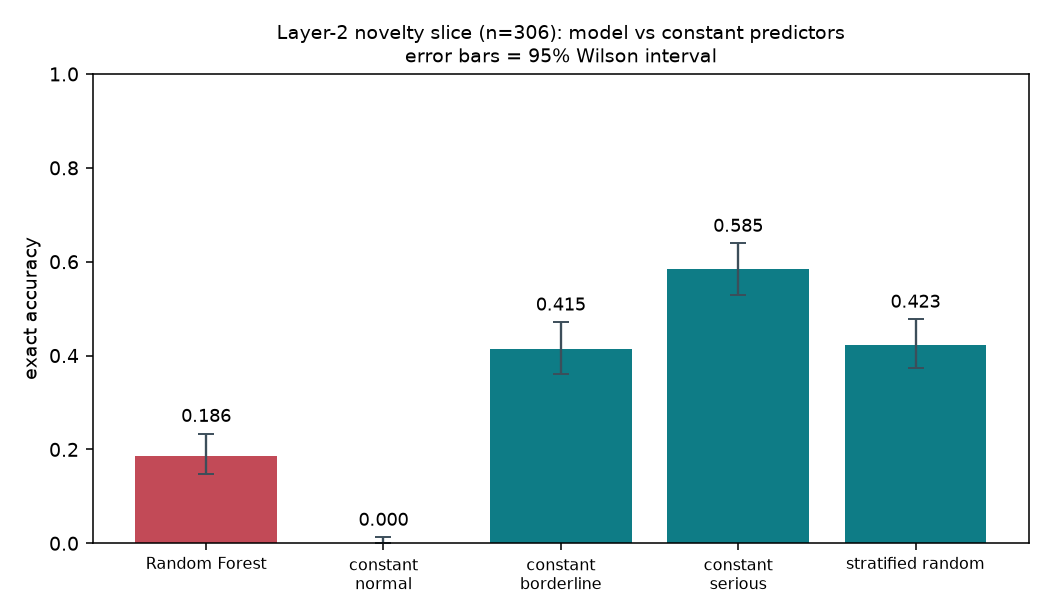
\includegraphics[width=0.85\linewidth]{novelty_baselines}
	\caption{\textbf{Model versus constant predictors on the novelty slice.}
    The learned model (left) falls well below every non-degenerate constant
    baseline. Error bars are 95\% Wilson intervals. The rule engine scores zero here
    by construction, since the slice is defined as the set of records on which the
    rules are wrong.}\label{fig:baselines}
\end{figure}

Against the strongest constant baseline the model wins on 47 records and loses on
169 (exact McNemar $p = 2.4\times10^{-17}$): it is significantly \emph{worse} than
predicting a single class. Aggregate metrics on the same model are nonetheless
strong --- accuracy 0.889, macro-F1 0.867, ROC-AUC 0.973 --- which is precisely
the dissociation H1 predicts.

Two further pilot findings identify the mechanism. First, the model reproduces the
Layer-1 rule output on 93.5\% of test records, and 97.4\% of its \texttt{serious}
predictions fall on records the rules had already flagged --- across the whole test
set it makes only 29 \texttt{serious} calls the rules did not. Second, Layer~1 can
never be \texttt{serious} on the novelty slice, because the slice is defined as
Layer~2 $>$ Layer~1 and \texttt{serious} is the maximum class. A model that has
learned Layer~1 is therefore structurally incapable of raising \texttt{serious}
there, whatever the biomarkers show; it recovers 10 of 179 such cases. The ceiling
on the experiment was fixed by the label design before any model was trained.

The competing explanation --- that medication normalises the analytes and so erases
the signal --- is \emph{not} supported. Accuracy is no higher among unmedicated
records (Fisher $p = 0.549$), and treated panels read \emph{less} normal under the
rule engine (29.4\%) than antihypertensive-only (77.1\%) or unmedicated (69.2\%)
panels, which is the opposite of what erasure predicts.

Table~\ref{tab:fusion} reports the cost of admitting the model to the pipeline.

\begin{table}[h!]
\centering
\caption{Pilot: effect of adding the model to the rule engine, over the full test
set ($n = 3862$).\label{tab:fusion}}
\renewcommand{\arraystretch}{1.15}
\begin{tabular}{|l|c|}
\hline
\textbf{Quantity} & \textbf{Value} \\
\hline
Rule engine alone, accuracy      & 0.9208 [0.9118, 0.9289] \\
Model alone, accuracy            & 0.8887 [0.8783, 0.8982] \\
Fused $\max(\text{rule},\text{model})$, accuracy & 0.9184 [0.9094, 0.9267] \\
\hline
Records the model repairs        & 57 \\
Records the model damages        & 66 \\
Net effect                       & $-9$ (exact McNemar $p = 0.47$) \\
\hline
False escalations (non-novelty)  & 66 / 3556 = 1.86\% [1.46, 2.35] \\
\quad of which normal $\to$ borderline & 47 \\
\quad of which borderline $\to$ serious & 19 \\
Warranted escalations that overshot & 0 \\
\hline
\end{tabular}
\end{table}

The model's contribution to system accuracy is not distinguishable from zero and
the point estimate is negative. One reassuring detail: where escalation was
warranted the model never overshot, so all the harm is escalation that was not
needed rather than over-escalation where some was.

A fourth observation concerns the evaluation instruments themselves. Rule-engine
accuracy is 0.9208, and $3556/3862 = 0.9208$ exactly --- the figure is
definitionally the proportion of records Layer~2 does not upgrade, not a
performance measure. Together with the inflated ROC-AUC, a risk-detection rate that
any constant non-normal predictor saturates, and a groundedness score computed
after ungrounded items have been deleted, this gives four independent instances of
the same failure: a metric that cannot report a negative result. Cataloguing them
is a secondary contribution of the project.

Retrieval attains P@1 $=0.857$ and P@3 $=0.667$ on the silver standard. Generation
over five test patients produced 38 advice items with zero diagnostic violations
and no parse failures. Report ingestion was tested against two real laboratory PDFs
of differing house style, recovering 24 of 24 and 27 analytes respectively, with
patient age and sex read correctly from both headers.

\subsection{Threats to validity}

\textbf{Internal.} The dominant threat is the label--feature coupling that RQ1
exists to characterise; it is addressed by making it the object of study rather
than a caveat. Layer-2 labels derive from self-reported questionnaire responses and
therefore carry measurement error, so an unknown share of the residual error is
label noise rather than model failure --- a limitation that cannot be resolved with
this dataset and will be stated as such.

\textbf{External.} The model is trained on US survey data and labelled with UK
guideline thresholds; the population and the guidance do not correspond. Survey
weights are not applied, so results describe the sample rather than the US
population. Neither is corrected, and both bound the generalisability claims that
may be made.

\textbf{Construct.} The retrieval gold standard is derived from the corpus's own
metadata, and the corpus is small. The faithfulness proxy is an embedding
similarity threshold, not an entailment judgement. Both measure something weaker
than the construct named, and are reported with that qualification attached.

\textbf{Statistical.} The novelty slice contains 306 records, so interval estimates
are wide; all proportions are therefore reported with confidence intervals and no
claim rests on a point estimate alone.

\subsection{Success criteria}

The project succeeds if it delivers: (i) a reproducible dataset and labelling
procedure; (ii) a working end-to-end system; (iii) a defensible answer to RQ1
supported by baselines and interval estimates, \emph{whether that answer is
positive or negative}; and (iv) an honest account of the limits of the evaluation
instruments themselves. A negative answer to RQ1, properly evidenced, is an
acceptable and indeed anticipated outcome.

%%%%%%%%%%%%%%%%%%%%%%%%%%%%%%%%%%%%%%%%%%%%%%%%%%%%%%%%%%%%%%%%%%%%%%
\section{Project management}

\subsection{Work breakdown and schedule}

\begin{table}[h!]
\centering
\caption{Work packages, deliverables and due weeks.\label{tab:wp}}
\renewcommand{\arraystretch}{1.1}
\setlength{\tabcolsep}{4pt}
\begin{tabular}{|c|p{5.0cm}|p{6.6cm}|c|}
\hline
\textbf{WP} & \textbf{Task} & \textbf{Deliverable} & \textbf{Week} \\
\hline
1 & Literature review and scoping & Annotated bibliography; proposal & 1--3 \\
2 & Data acquisition and preparation & Reproducible pipeline; processed dataset & 3--5 \\
3 & Rule engine and label construction & Configurable ruleset; labelled dataset & 5--6 \\
4 & Model training and interpretability & Trained model; SHAP analysis & 6--8 \\
5 & Retrieval corpus and index & Cited corpus; FAISS index & 8--9 \\
6 & Generation and safety guards & Generator; groundedness verifier & 9--11 \\
7 & Interfaces (dashboard, API) & Local application; documented API & 11--12 \\
8 & Report ingestion (RQ3) & Layout-agnostic parser; regression tests & 12--13 \\
9 & Evaluation and baselines (RQ1, RQ2) & Metrics, figures, statistical tests & 13--15 \\
10 & Dissertation write-up & Final report & 15--18 \\
\hline
\end{tabular}
\end{table}

Progress is tracked through version control, with each work package producing a
committed, testable artefact. An automated test suite runs on every change, so
regressions are detected at the point of introduction rather than at the end.

\subsection{Risk register}

\begin{table}[h!]
\centering
\caption{Principal risks and mitigations.\label{tab:risk}}
\renewcommand{\arraystretch}{1.1}
\setlength{\tabcolsep}{4pt}
\begin{tabular}{|p{4.4cm}|c|c|p{7.4cm}|}
\hline
\textbf{Risk} & \textbf{Lik.} & \textbf{Imp.} & \textbf{Mitigation} \\
\hline
Model shown to add no value & High & Med & Reframe as a methodological result; the negative finding is itself the contribution. Anticipated from the outset. \\
\hline
Hosted LLM unavailable or model slug retired & High & Med & Provider abstraction with a fully local option; pipeline degrades to assessment-only; model name and access date recorded. \\
\hline
Evaluation metrics cannot fail by construction & Med & High & Explicit audit of each metric for degeneracy; report pre-filter as well as post-filter figures. \\
\hline
Guideline corpus too small to generalise & High & Med & State as a limitation; report retrieval metrics with the corpus size prominent. \\
\hline
PDF layouts defeat the parser & Med & Med & Manual review step mandatory before analysis; CSV/JSON always available as reliable fallback. \\
\hline
Compute constraints (CPU-only, 16\,GB) & Med & Low & Tree-based model and small embedding model chosen deliberately; no GPU dependency anywhere. \\
\hline
Scope creep from engineering work & High & Med & Feature freeze at WP9; remaining time reserved for evaluation and writing. \\
\hline
\end{tabular}
\end{table}

\subsection{Ethical, legal and regulatory considerations}

\textbf{Human participants and data.} No human participants are recruited and no
personal data is collected. NHANES is a public, de-identified dataset released for
secondary analysis under its published terms, which removes the need for primary
ethics approval. Any blood-report documents used to test ingestion are the author's
own or synthetic, are not committed to version control, and are not redistributed.

\textbf{Regulatory boundary.} A system that produces health guidance from clinical
measurements approaches the boundary of software as a medical device. The project
is positioned firmly on the non-diagnostic side: no diagnosis, no medication or
dosing advice, no triage decision. This positioning is enforced structurally rather
than by intention alone --- there is no diagnosis field in the output schema, a
guard scans generated text for diagnostic phrasing, and a fixed disclaimer is
system-owned. An intended-use statement will be included in the final report. It is
acknowledged that the non-diagnostic guard is a mitigation, not a validated control.

\textbf{Data flow and confidentiality.} Rule evaluation, model inference, retrieval
and report parsing execute entirely locally. Where a hosted language model is used
for generation, the request contains age, sex and biomarker values only; no name,
address or identifier is transmitted. A fully local generation option is provided
for users unwilling to accept even that disclosure. This is documented in the
user-facing materials.

\textbf{Risk of harm.} The foreseeable harms are a false reassurance (mitigated by
the safety-dominant fusion, which cannot lower a rule-based finding) and
unnecessary alarm (quantified directly as the false-escalation rate). Guidance is
confined to lifestyle measures for which the evidence base is broad and the
downside of a mistaken recommendation is small.

\textbf{Attribution.} Guideline content is paraphrased with source and code
attribution rather than reproduced, respecting the publishers' terms.

\subsection{Resources}

All resources are freely available: NHANES data from the CDC; NICE, NHS and WHO
guidance from their public sites; Python with open-source scientific libraries; a
consumer laptop (16\,GB RAM, CPU-only). Language-model access uses a free-tier
hosted provider with a local fallback. No proprietary datasets, licensed software
or specialised hardware are required, so no resource dependency threatens delivery.

%%%%%%%%%%%%%%%%%%%%%%%%%%%%%%%%%%%%%%%%%%%%%%%%%%%%%%%%%%%%%%%%%%%%%%
\section{Conclusion}

This proposal describes a system that turns a blood-test report into cited,
non-diagnostic lifestyle guidance, and --- more importantly --- an investigation
that the system makes possible. The intended contribution is a demonstrated
procedure for deciding whether a learned component earns its place when the
supervised label has been constructed from rules applied to that component's own
inputs.

The pilot results reported in Section~4.6 indicate that the answer, for this
system, is likely to be negative: the model reproduces the rule engine on the great
majority of records, fails to exceed a constant predictor on the only subpopulation
where the label carries independent information, and produces no measurable net
improvement to the fused output. Establishing that cleanly, with baselines,
interval estimates and an identified mechanism, is a more useful result than an
unexamined ROC-AUC of 0.97 --- and it generalises well beyond this application, to
any clinical prediction task whose labels are defined by thresholds on its own
predictors.

\newpage
%%%%%%%%%%%%%%%%%%%%%%%%%%%%%%%%%%%%%%%%%%%%%%%%%%%%%%%%%%%%%%%%%%%%%%
\addcontentsline{toc}{section}{References}

\newcommand{\bibspace}[0]{\vspace*{0.1cm}}
\begin{thebibliography}{99}

\bibitem{breiman2001random}
Breiman, L.,
\newblock ``{Random Forests},''
\newblock \emph{Machine Learning}, vol.~45, no.~1, pp.~5--32, 2001.

\bibspace
\bibitem{cdc2021nhanes}
Centers for Disease Control and Prevention, National Center for Health Statistics,
\newblock ``{National Health and Nutrition Examination Survey (NHANES) Data,
2013--2020},''
\newblock Hyattsville, MD, U.S. Department of Health and Human Services.

\bibspace
\bibitem{collins2015tripod}
Collins, G.~S., Reitsma, J.~B., Altman, D.~G., and Moons, K.~G.~M.,
\newblock ``{Transparent Reporting of a multivariable prediction model for
Individual Prognosis or Diagnosis (TRIPOD): the TRIPOD statement},''
\newblock \emph{BMJ}, vol.~350, g7594, 2015.

\bibspace
\bibitem{es2024ragas}
Es, S., James, J., Espinosa-Anke, L., and Schockaert, S.,
\newblock ``{RAGAS: Automated Evaluation of Retrieval Augmented Generation},''
\newblock in \emph{Proc. European Chapter of the ACL (EACL): System
Demonstrations}, 2024.

\bibspace
\bibitem{ji2023hallucination}
Ji, Z., Lee, N., Frieske, R., Yu, T., Su, D., Xu, Y., Ishii, E., Bang, Y.~J.,
Madotto, A., and Fung, P.,
\newblock ``{Survey of Hallucination in Natural Language Generation},''
\newblock \emph{ACM Computing Surveys}, vol.~55, no.~12, pp.~1--38, 2023.

\bibspace
\bibitem{johnson2019faiss}
Johnson, J., Douze, M., and J\'egou, H.,
\newblock ``{Billion-scale similarity search with GPUs},''
\newblock \emph{IEEE Transactions on Big Data}, vol.~7, no.~3, pp.~535--547, 2019.

\bibspace
\bibitem{kaufman2012leakage}
Kaufman, S., Rosset, S., Perlich, C., and Stitelman, O.,
\newblock ``{Leakage in Data Mining: Formulation, Detection, and Avoidance},''
\newblock \emph{ACM Transactions on Knowledge Discovery from Data}, vol.~6, no.~4,
pp.~1--21, 2012.

\bibspace
\bibitem{lewis2020rag}
Lewis, P., Perez, E., Piktus, A., Petroni, F., Karpukhin, V., Goyal, N.,
K\"uttler, H., Lewis, M., Yih, W., Rockt\"aschel, T., Riedel, S., and Kiela, D.,
\newblock ``{Retrieval-Augmented Generation for Knowledge-Intensive NLP Tasks},''
\newblock in \emph{Advances in Neural Information Processing Systems (NeurIPS)},
2020.

\bibspace
\bibitem{lundberg2017shap}
Lundberg, S.~M., and Lee, S.-I.,
\newblock ``{A Unified Approach to Interpreting Model Predictions},''
\newblock in \emph{Advances in Neural Information Processing Systems (NeurIPS)},
2017.

\bibspace
\bibitem{mcnemar1947note}
McNemar, Q.,
\newblock ``{Note on the sampling error of the difference between correlated
proportions or percentages},''
\newblock \emph{Psychometrika}, vol.~12, no.~2, pp.~153--157, 1947.

\bibspace
\bibitem{reimers2019sbert}
Reimers, N., and Gurevych, I.,
\newblock ``{Sentence-BERT: Sentence Embeddings using Siamese BERT-Networks},''
\newblock in \emph{Proc. Conference on Empirical Methods in Natural Language
Processing (EMNLP)}, 2019.

\bibspace
\bibitem{roberts2021common}
Roberts, M., Driggs, D., Thorpe, M., et al.,
\newblock ``{Common pitfalls and recommendations for using machine learning to
detect and prognosticate for COVID-19 using chest radiographs and CT scans},''
\newblock \emph{Nature Machine Intelligence}, vol.~3, pp.~199--217, 2021.

\bibspace
\bibitem{rudin2019stop}
Rudin, C.,
\newblock ``{Stop explaining black box machine learning models for high stakes
decisions and use interpretable models instead},''
\newblock \emph{Nature Machine Intelligence}, vol.~1, pp.~206--215, 2019.

\bibspace
\bibitem{saito2015precision}
Saito, T., and Rehmsmeier, M.,
\newblock ``{The Precision-Recall Plot Is More Informative than the ROC Plot When
Evaluating Binary Classifiers on Imbalanced Datasets},''
\newblock \emph{PLoS ONE}, vol.~10, no.~3, e0118432, 2015.

\bibspace
\bibitem{wilson1927probable}
Wilson, E.~B.,
\newblock ``{Probable Inference, the Law of Succession, and Statistical
Inference},''
\newblock \emph{Journal of the American Statistical Association}, vol.~22,
no.~158, pp.~209--212, 1927.

\bibspace
\bibitem{wynants2020prediction}
Wynants, L., Van Calster, B., Collins, G.~S., et al.,
\newblock ``{Prediction models for diagnosis and prognosis of covid-19: systematic
review and critical appraisal},''
\newblock \emph{BMJ}, vol.~369, m1328, 2020.

\end{thebibliography}

\newpage
%%%%%%%%%%%%%%%%%%%%%%%%%%%%%%%%%%%%%%%%%%%%%%%%%%%%%%%%%%%%%%%%%%%%%%
\appendix
\section*{Appendix A: Biomarker panel}
\addcontentsline{toc}{section}{Appendix A}

The rule engine evaluates 27 analytes across six panels. Twenty-one are
\emph{actionable} (they drive both the severity label and lifestyle guidance) and
six are \emph{flag-only} (reported and able to raise an urgent referral, but never
attracting lifestyle advice, and excluded from the model).

\begin{table}[h!]
\centering
\renewcommand{\arraystretch}{1.1}
\begin{tabular}{|l|p{11.5cm}|}
\hline
\textbf{Panel} & \textbf{Analytes} \\
\hline
Cardiometabolic & HbA1c, fasting glucose, total cholesterol, LDL, HDL, triglycerides \\
\hline
Complete blood count & haemoglobin, haematocrit, RBC, MCV, MCH, MCHC, RDW, WBC\textsuperscript{*}, platelets\textsuperscript{*} \\
\hline
Liver & ALT, AST, ALP, albumin, total bilirubin \\
\hline
Kidney & creatinine, urea nitrogen \\
\hline
Electrolytes & sodium\textsuperscript{*}, potassium\textsuperscript{*}, chloride\textsuperscript{*}, calcium\textsuperscript{*} \\
\hline
Vitamins & vitamin D \\
\hline
\end{tabular}
\end{table}

\noindent{\footnotesize \textsuperscript{*}Flag-only: reported and able to raise an
urgent referral, but never used for lifestyle advice and excluded from the model's
feature matrix.}

\end{document}
